\chapter{Reti Neurali Artificiali: le basi} % Main chapter title

\label{Capitolo1} % Change X to a consecutive number; for referencing this chapter elsewhere, use \ref{ChapterX}
%variables to define path to images
\def \path {Figures/C1}
\def \teoria {Figures/teoria}

%--------------------------------------------------------------------%--------------------
%	SECTION 1
%--------------------
%--------------------------------------------------------------------

\section{Breve introduzione}
\label{sec:intro}
%COSA SONO LE RETI NEURALI ARTIFICIALI
Una rete neurale artificiale – chiamata normalmente solo rete neurale (in inglese \emph{Neural Network}) – è
un modello di calcolo adattivo, ispirato ai principi di funzionamento del sistema nervoso degli organismi evoluti che secondo l'approccio connessionista\parencite{WConnessionismo} possiede una complessità non descrivibile con i metodi simbolici.  
La caratteristica fondamentale di una rete neurale è che essa è capace di acquisire conoscenza modificando la propria struttura in base alle informazioni esterne (i dati in ingresso) e interne (tramite le connessioni) durante il processo di apprendimento. Le informazioni sono immagazzinate nei parametri della rete, in particolare, nei pesi associati alle connessioni. 
Sono strutture non lineari in grado di simulare relazioni complesse tra
ingressi e uscite che altre funzioni analitiche non sarebbero in grado di fare. 


L'unità base di questa rete è il neurone artificiale introdotto per la prima volta da McCulloch e
Pitts nel 1943 (fig. \ref{fig:neuron}).


\begin{figure}[h!]
 \centering
 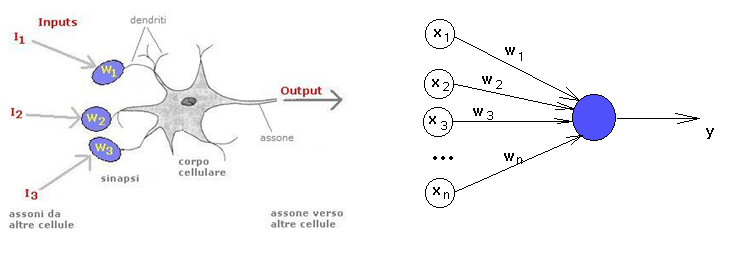
\includegraphics[width=1.0\textwidth]{\teoria/NeuronePitts.png}
 \caption{Modello di calcolo di un neurone (a sinistra) e schema del neurone artificiale (a destra)}
 \label{fig:neuron}
\end{figure}

Si tratta di un'unità di calcolo a N ingressi e 1 uscita. Come si può vedere dall'immagine a
sinistra gli ingressi rappresentano le terminazioni sinaptiche, quindi sono le uscite di altrettanti
neuroni artificiali. A ogni ingresso corrisponde un peso sinaptico $w$, che stabilisce quanto quel
collegamento sinaptico influisca sull'uscita del neurone. Si determina quindi il potenziale del neurone facendo una somma degli ingressi, pesata secondo i pesi $w$. \\
A questa viene applicata una funziona di trasferimento non lineare: 
\begin{equation}
 f(x) = H(\sum_{i}(w_i x_i))
\end{equation} 
ove $H$ è la funzione gradino di Heaviside \parencite{WHeaviside}. Vi sono, come vedremo, diverse altre funzioni non lineari tipicamente utilizzate come funzioni di attivazioni dei neuroni. 
Nel '58 Rosenblatt propone il modello di \emph{Percettrone} rifinendo il modello di neurone a soglia, aggiungendo un termine di \emph{bias} e un algoritmo di apprendimento basato sulla minimizzazione dell'errore, cosiddetto \emph{error back-propagation}\parencite{WPercettrone}.
\begin{equation}
 f(x) = H(\sum_{i}(w_i x_i)+b),\quad ove \quad b = bias \\
\end{equation}
\begin{equation} 
 w_i(t+1) = w_i(t)+\eta \delta x_i(t)
\end{equation}
dove $\eta$ è una costante di apprendimento strettamente positiva che regola la velocità di apprendimento, detta \emph{learning rate} e $\delta$ è la discrepanza tra l'output desiderato e l'effettivo output della rete. 

Il percettrone però era in grado di imparare solo funzioni linearmente separabili. Una maniera per oltrepassare questo limite è di combinare insieme le risposte di più percettroni, secondo architetture multistrato. 
%--------------------------------------------------------------------%--------------------
%	SECTION 2
%--------------------
%--------------------------------------------------------------------

\section{Multi-layer Perceptron}
\label{sec:mlp}
Il Multi-layer Perceptron (\textit{MLP}) o percettrone multi-strato è un tipo di rete feed-forward che mappa un set di input ad un set di output. È la naturale estensione del percettrone singolo e permette di distinguere dati non linearmente separabili.

\begin{figure}[h!]
 \centering
 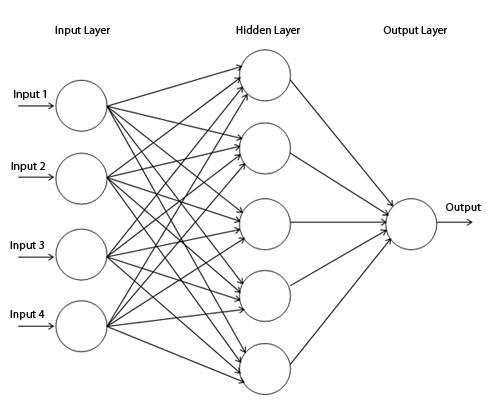
\includegraphics[width=1.0\textwidth]{\teoria/multilayer.png}
 \caption{Struttura di un percettrone multistrato con un solo strato nascosto}
 \label{fig:multilayer}
\end{figure}


Il \emph{mlp} possiede le seguenti caratteristiche: 
\begin{itemize}
\item ogni neurone è un percettrone come quello descritto nella sezione \ref{sec:intro}. Ogni unità possiede quindi una propria funzione d'attivazione non lineare.
\item a ogni connessione tra due neuroni corrisponde un peso sinaptico $w$
\item è formato da 3 o più strati. In \ref{fig:multilayer} è mostrato un MLP con uno strato di input; un solo strato nascosto (o \emph{hidden layer}; ed uno di output.) 
\item l'uscita di ogni neurone dello strato precedente è l'ingresso per ogni neurone dello
strato successivo. È quindi una rete \emph{completamente connessa}. Tuttavia, si possono
disconnettere selettivamente settando il peso sinaptico $w$ a 0.
\item la dimensione dell'input e la dimensione dell'output dipendono dal numero di
neuroni di questi due strati. Il numero di neuroni dello strato nascosto è invece
indipendente, anche se influenza di molto le capacità di apprendimento della rete. 
\end{itemize}
%non linearità 
Se ogni neurone utilizzasse una funzione lineare allora si potrebbe ridurre l'intera rete ad una composizione di funzioni lineari. Per questo - come detto prima - ogni neurone possiede una funzione di attivazione non lineare. 

%black box
\subsection{Strati Nascosti}
I cosiddetti \emph{hidden layers} sono una parte molto interessante della rete. Per il teorema di
approssimazione universale\parencite{WApprox}, \cite{WApprox} \parencite{WConnessionismo} una rete con un singolo strato nascosto e un numero finiti di
neuroni, può essere addestrata per approssimare una qualsiasi funzione continua su uno spazio compatto di $\mathbb{R}^n$. In altre parole, un singolo strato nascosto è abbastanza potente da imparare un ampio numero di funzioni. Precisamente, una rete a 3 strati è in grado di separare regioni convesse con un numero di lati $\leqslant$ numero neuroni nascosti. 

Reti con un numero di strati nascosti maggiore di 3 vengono chiamate reti neurali profonde o \emph{deep neural network}; esse sono in grado di separare regioni qualsiasi, quindi di approssimare praticamente qualsiasi funzione. Il primo e l’ultimo strato devono avere un numero di neuroni pari alla dimensione dello spazio di ingresso e quello di uscita. Queste sono le terminazioni della \emph{"black box"} che rappresenta la funzione che vogliamo approssimare. 

L'aggiunta di ulteriori strati non cambia \emph{formalmente} il numero di funzioni che si possono approssimare; tuttavia vedremo che nella pratica un numero elevato di strati migliori di gran lunga le performance della rete su determinati task, essendo gli hidden layers gli strati dove la rete memorizza la propria rappresentazione astratta dei dati in ingresso. Nel capitolo 4 vedremo un'architettura all'avanguardia con addirittura 152 strati.
 
%--------------------------------------------------------------------%--------------------
%	SECTION 3
%--------------------
%--------------------------------------------------------------------

\section{Caso di studio: prevedere il profitto di un ristorante}
%%%  30 Coperti - 11 Mesi all'anno
%%%  20 coperti - 38-42 ore di apertura a settimana 
%%%  Profitto in % = Ricavo - Spesa, According to the Restaurant Resource Group, average profit margins for restaurants range from 2 to 6 percent. 
%%% 
Prendendo spunto dalla traccia d'esame di Sistemi Intelligenti M del 2 Aprile 2009: \\
\textit{"Loris è figlio della titolare di una famoso spaccio di piadine nel Riminese e sta tornando in Italia
dopo aver frequentato con successo un prestigioso Master in Business Administration ad Harvard, a
cui si è iscritto inseguendo il sogno di esportare in tutto il mondo la piadina romagnola. Nel lungo
viaggio in prima classe, medita su come presentare alla mamma, che sa essere un tantino restia alle
innovazioni, il progetto di aprire un ristorantino a New York City."}

Loris ha esportato con successo la piadina a NY, si veda \parencite{WGradisca} \href{www.gradiscanyc.com} ma col passare degli anni ha notato alcuni problemi e vuole utilizzare di nuovo le sue brillanti capacità analitiche per migliorare il profitto del suo ambizioso ristorante. \\
I problemi sono 2: 
\begin{enumerate}
\item il ristorante è conosciuto ormai - si sa che tutti vogliono mangiare italiano - ma il numero dei coperti era rimasto a 22, come quelli iniziali; 
\item gli orari di apertura sono troppo lunghi e vi sono alcune zone morte dove il costo di mantenere aperto il ristorante è maggiore rispetto al ricavo dei pochi clienti che si siedono a mangiare durante quelle ore; 
\end{enumerate}
Secondo la National Restaurant Association\parencite{WProfit} \parencite{WRRG} il profitto medio lordo annuo di un ristorante negli Stati Uniti varia dal 2 al 6\%. Così Loris ha collezionato alcuni dati riguardo gli ultimi anni e - attratto da tutta quest'entusiasmo attorno alle reti neurali - decide di provare ad utilizzarle per trovare il trade-off ottimale di coperti e di orari di apertura settimanali per massimizzare il profitto del suo ristorante. 

%--------------------------------------------------------------------%--------------------
%	SECTION 4
%--------------------
%--------------------------------------------------------------------

\section{Implementazione da zero di un MLP}
%Parlare brevemente del caso di studio
Per il suddetto caso di studio si è implementato da zero un percettrone multistrato a 3 strati come quello illustrato in sezione \ref{sec:mlp}. Vediamo qui di seguito le varie parti da implementare passo passo per costruire un MLP, addestrarlo e testare che l'addestramento sia stato eseguito in maniera corretta. Il progetto è realizzato in Lua, per sfruttare il framework per il \emph{Machine Learning} Torch\ref{Capitolo3}
\subsection{Dataset e Architettura}
Nei vari anni, Loris ha cambiato le due variabili in gioco annotando di volta in volta i risultati. Siccome i coperti erano troppo pochi e le file d'attesa erano troppo lunghe, il ristorante perdeva alcuni clienti. Quindi Loris ha portato i coperti a 25 e diminuendo le ore settimanali a 38, ed i profitti sono aumentati. Tuttavia, non era raro che ancora qualche cliente dovesse aspettare in piedi per troppo tempo (si sa la vita a NY è frenetica), finendo poi per scegliere un ristorante adiacente. Inoltre, aveva diminuito le ore di troppo; nel weekend i clienti arrivavano fino a tardi, quindi rimanere aperti un'ora in più sarebbe stato lungimirante. Così, dopo l'allargamento della sala principale, ha aggiunto altri coperti ed aumentato le ore settimanali a 40, segnando un record personale di $4.4\%$ di profitti annui. \\

Quindi, i dati in ingresso ed in uscita, in $X$ e $Y$ rispettivamente sono:
\[ 
X = \begin{pmatrix}
22 & 42\\ 
25 & 38 \\ 
30 & 40
\end{pmatrix} 
%
Y = \begin{pmatrix}
2.8\\ 
3.4 \\ 
4.4
\end{pmatrix} 
\]
Osservando le dimensioni dei dati si nota che la rete deve avere 2 input e dare in uscita 1 output, che chiameremo $\hat{y}$, in contrapposizione a $y$ che è l'uscita desiderata. Per quanto detto nella sezione \ref{sec:mlp}, il MLP deve avere 2 neuroni nello strato di ingresso ed 1 solo in uscita. Per quanto riguarda lo strato nascosto, la rete avrà 3 neuroni. Questi parametri vengono chiamati \emph{hyperparameters}. In figura \ref{fig:mlp} è mostrata l'architettura generale della nostra rete. 

\begin{figure}[h!]
 \centering
 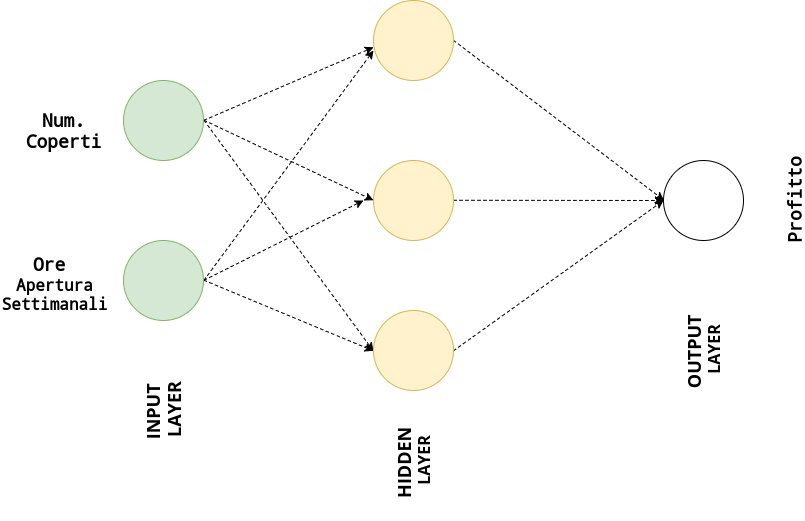
\includegraphics[width=1.0\textwidth]{\path/MLP-Profitto.png}
 \caption{Struttura di un percettrone multistrato con un solo strato nascosto}
 \label{fig:mlp}
\end{figure}

\subsection{Modello Neurone \& Forward Propagation}
\subsection{Backpropagation}
Come si fa ad addestrare una rete multistrato con diversi neuroni per strato? Tramite l'algoritmo di \emph{backpropagation of errors} di ... 
\subsection{Verifica numerica del gradiente}
\subsection{Addestramento}

%--------------------------------------------------------------------%--------------------
%	SECTION 5
%--------------------
%--------------------------------------------------------------------

\section{Ottimizzazione: diverse tecniche}
%SGD ASGD LBGFS ADAM 
%INSERIRE GRAFICI 


%--------------------------------------------------------------------%--------------------
%	SECTION 6
%--------------------
%--------------------------------------------------------------------
\section{Overfitting: come rilevarlo e risolverlo}



%--------------------------------------------------------------------%--------------------
%	SECTION 7
%--------------------
%--------------------------------------------------------------------

\section{Risultati}
